\documentclass{article}
\usepackage[utf8]{inputenc}
\usepackage[margin=1.2in]{geometry}
\usepackage{hyperref}
\usepackage{listings}
\usepackage{xcolor}
\usepackage{minted}


\usepackage{tikz}
\usetikzlibrary{positioning}

\usepackage{natbib}
\usepackage{graphicx}
\usepackage{amsmath}

\title{\vspace{-2 cm}Universidade Federal de Ouro Preto \\ Inteligência Artificial \\ Prova 1}
\author{Prof. Rodrigo Silva}
\date{}


\begin{document}

\maketitle


\begin{enumerate}
    
    \item Considere o problema de encontrar um caminho no labirinto abaixo. O objetivo é ir da posição \textbf{s} até a posição \textbf{g}. O agente pode se mover horizontalmente e verticalmente. 
    
    \begin{enumerate}
        
        \item (1pt) No labirinto abaixo, numere os nós expandidos (visitados) por um agente que implementa o algoritmo de busca e profundidade. A ordem das ações é para cima, para a esquerda, para a direita, e para baixo. Assuma poda de ciclos.
        \begin{figure}[!ht]
            \centering
            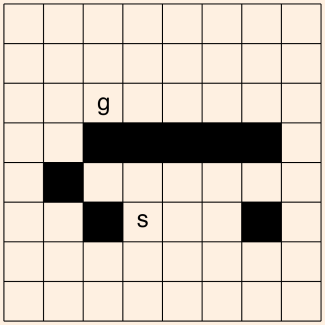
\includegraphics[width=0.42\textwidth]{grid.png}
        \end{figure}
        
        \item (1pt) No labirinto abaixo, escreva em cada nó o valor da heurística do nó, considerando a distância de Manhattan. Considere que cada quadrado tem lado 1 u.m.
        \begin{figure}[!ht]
            \centering
            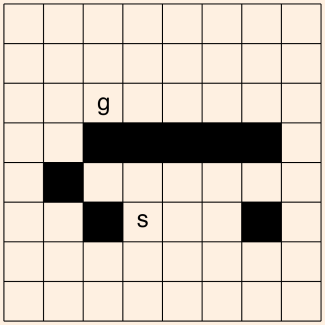
\includegraphics[width=0.42\textwidth]{grid.png}
        \end{figure}
        
        \pagebreak
        \item (1pt) No labirinto abaixo, numere os nós expandidos (visitados) por um agente que implementa um algoritmo guloso pela heurística calculada acima.
        \begin{figure}[!ht]
            \centering
            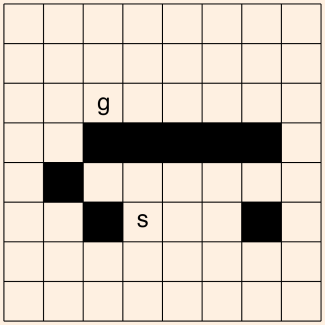
\includegraphics[width=0.42\textwidth]{grid.png}
        \end{figure}
        
        \vspace{2cm}
        
        \item (1pt) No labirinto abaixo, numere os nós expandidos (visitados) por um agente que implementa o algoritmo $A^*$ considerando a distância de Manhattan como custo e heurística.
        \begin{figure}[!ht]
            \centering
            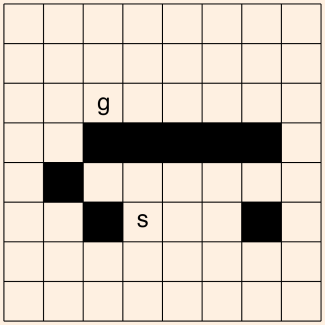
\includegraphics[width=0.42\textwidth]{grid.png}
        \end{figure}
        
    \end{enumerate}
    
    \pagebreak
    
    \item Considere o problema das n-Rainhas.
    
    \begin{enumerate}
        \item (1pt) Apresente uma formulação eficiente do problema, como um problema de satisfação de restrições.
    
    \begin{tikzpicture}
    \draw (0,0) -- (14,0) -- (14,8) -- (0,8) -- (0,0);
    \end{tikzpicture}
    
    \vspace{1.5cm}
        \item (1pt) Apresente a rede (grafo) de restrições considerando o problema das \textbf{3-rainhas}.
        
    \begin{tikzpicture}
    \draw (0,0) -- (14,0) -- (14,8) -- (0,8) -- (0,0);
    \end{tikzpicture}
        
    \end{enumerate}
    
    \pagebreak    
    \item Considere o CSP abaixo:

        \begin{align*}
        X &= \{A,B,C\} \\
        D &= \{\{1,2,3,4\},\{1,2,3,4\},\{1,2,3,4\} \}\\
        C &= \{ A = B, B > C \}    
        \end{align*}

    \begin{enumerate}
        \item (1pt) Apresente a rede (grafo) de restrições do problema.  
        
        \begin{tikzpicture}
    \draw (0,0) -- (14,0) -- (14,4) -- (0,4) -- (0,0);
    \end{tikzpicture}
        
        \item (1pt) Apresente o estado da lista $to\_do$ a cada iteração do algoritmo apresentado na Figura \ref{fig:GAC}. 
            \begin{figure}[!ht]
            \centering
            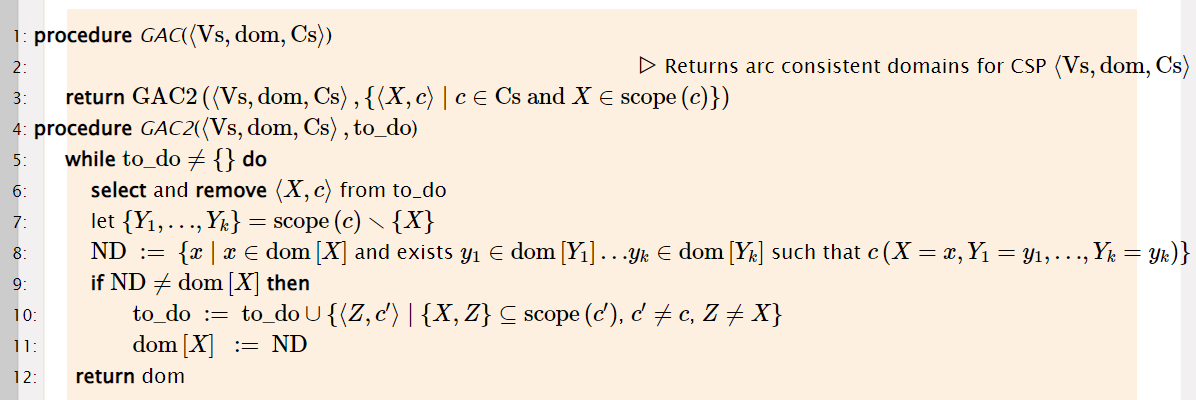
\includegraphics[width=1\textwidth]{gac.png}
            \label{fig:GAC}
            \end{figure}
            
        \begin{tikzpicture}
        \draw (0,0) -- (14,0) -- (14,7) -- (0,7) -- (0,0);
     \end{tikzpicture}
        
    \end{enumerate}
    
    \pagebreak

    \item Considere a seguinte base de conhecimento (KB):
    
    \begin{center}
        \begin{align*}
         a & \leftarrow b \wedge c. \\ 
         b & \leftarrow e. \\ 
         b & \leftarrow d. \\ 
         c &. \\ 
         d & \leftarrow h. \\ 
         e &. \\
         g & \leftarrow a \wedge b  \wedge e. \\
         f & \leftarrow h \wedge b. \\  
        \end{align*}
    \end{center}
    
    
    \begin{enumerate}
        \item (1pt) Mostre como uma prova bottom-up para esta base de conhecimento. Apresente todas as consequências lógicas desta KB.
        
        \begin{tikzpicture}
        \draw (0,0) -- (14,0) -- (14,7) -- (0,7) -- (0,0);
     \end{tikzpicture}
        
        \item (1pt) Apresente uma prova top-down para a pergunta $ask$ $g$.
        
        \begin{tikzpicture}
        \draw (0,0) -- (14,0) -- (14,7) -- (0,7) -- (0,0);
     \end{tikzpicture}
        
    \end{enumerate}
    
\end{enumerate}




% Na leitura recomendada você deve ter lido que agentes são entidades que interagem com um ambiente. Nesta atividade você deve implementar agentes que encontram o caminho de uma posição inicial até uma posição alvo desviando de objetos. 

% Visite o repositório \url{https://github.com/rcpsilva/BCC740\_ArtificialIntelligence}, que contem o código base para esta atividade e leia atentamente o README.

% O arquivo \textit{Room.py} contém a classe \texttt{Room} que implementa um \texttt{Environment} que representa uma sala com obstáculos. Atributos importantes desta classe são:

% \begin{itemize}
%     \item \texttt{room}: É uma matriz que contém 0 nas posições livres e 0 nas posições com obstáculos.
%     \item \texttt{initial\_positon}: Posição inicial do agente na sala.
%     \item \texttt{target}: Posição em que o agente deve chegar.
% \end{itemize}

% O método de classe \texttt{initial\_percepts()} retorna:

% \begin{itemize}
%     \item \texttt{current\_position}: com a posição inicial do agente.
%     \item \texttt{target}: com a posição em que o agente deve chegar.
%     \item \texttt{neighboors} com as posições vizinhas livres. 
% \end{itemize}

% O método de classe \texttt{signal(action)} retorna:

% \begin{itemize}
%     \item \texttt{current\_position}: com a posição atual do agente.
%     \item \texttt{target}: com a posição em que o agente deve chegar.(Obs: Esta opção está aqui para modelar a possibilidade de mudança de objetivo durante a execução.)
%     \item \texttt{neighboors} com as posições vizinhas livres. 
% \end{itemize}

% Uma \texttt{action} é, da lista de vizinhos livres, a posição para onde o agente quer se mover. 

% Veja o exemplo ilustrado na figura \ref{fig:room}.

% \begin{figure}[!ht]
%     \centering
%     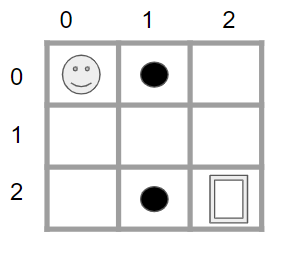
\includegraphics[width=0.4\textwidth]{room.PNG}
%     \caption{Ilustração da classe \texttt{Room}}
%     \label{fig:room}
% \end{figure}

% Para o exemplo mostrado na figura \ref{fig:room} teríamos:
%     \[
%         \texttt{room} = \begin{bmatrix}
%             0 & 1 & 0\\ 
%             0 & 0 & 0\\ 
%             0 & 1 & 0
%         \end{bmatrix}
%     \]
    
%     \[
%         \texttt{begin} = [0,0]
%     \]
    
%     \[
%         \texttt{target} = [2,2]
%     \]
    
%     \[
%         \texttt{current\_position} = [0,0]
%     \]
    
%     \[
%         \texttt{target} = [2,2]
%     \]
    
%     \[
%         \texttt{neighboors} = [[1,0],[1,1]]
%     \]

% o arquivo \textit{path\_finder\_agents.py} contém a implementação do \texttt{RandAgent}. Em cada posição, este agente escolhe um vizinho livre aleatoriamente para visitar. Ele para quando chega à posição alvo. Este agente pode ser usando como base para a implementação de outros agentes.

% Dadas estas informações, faça:

% \begin{enumerate}
%     \item Clone repositório \url{https://github.com/rcpsilva/BCC740\_ArtificialIntelligence}, leia atentamente o README e trabalhe a partir dele.
%     \item Execute o arquivo \textit{path\_finder\_simulation.py} para ver como o RandAgent se comporta.
%     \item No arquivo \textit{path\_finder\_agents.py}, implemente a classe \texttt{BFSAgent} que representa um agente que encontra a posição alvo fazendo uma busca em largura.
%     \item No arquivo \textit{path\_finder\_agents.py}, implemente a classe \texttt{DFSAgent} que representa um agente que encontra a posição alvo fazendo uma busca em profundidade.
%     \item No arquivo \textit{path\_finder\_agents.py}, implemente a classe \texttt{GreedyAgent} que representa um agente que encontra a posição alvo utilizando o algoritmo guloso.
%     \item No arquivo \textit{path\_finder\_agents.py}, implemente a classe \texttt{AStarAgent} que representa um agente que encontra a posição alvo utilizando o algoritmo A$^*$.
% \end{enumerate}

% Observações:
% \begin{itemize}
%     \item Todos os agentes implementados devem fazer poda de ciclos e poda de múltiplos caminhos.
%     \item Os agentes devem implementar a interface \texttt{Agent} definida no arquivo \textit{definitions.py}. 
%     \item Métodos auxiliares podem ser implementados para os agentes.
%     \item A classe $Room$ não deve ser modificada.
%     \item Os agentes implementados devem ser testados como indicado no arquivo \textit{path\_finder\_simulation.py}
% \end{itemize}
    

% %\bibliographystyle{plain}
% %\bibliography{references}
\end{document}

